\documentclass[11pt,a4paper]{article}

\usepackage[utf8]{inputenc}
\usepackage[margin=2.5cm]{geometry}
\usepackage{amsmath,amssymb,amsfonts}
\usepackage{mathtools}
\usepackage{siunitx}
\usepackage{threeparttable}
\usepackage{centernot}
\usepackage{multirow}
\usepackage{booktabs}
\usepackage{tabularx}
\usepackage{graphicx}
\usepackage{float}
\usepackage{url}
\usepackage{hyperref}
\hypersetup{hidelinks,hypertexnames=false}
\usepackage{cite}
\usepackage{caption}
\usepackage{microtype}
\usepackage{placeins}
\usepackage{needspace}
\usepackage{authblk}

% Pseudo-code packages
\usepackage{algorithm}
\usepackage{algpseudocode}

% Source-code listings
\usepackage{listings}

\newcommand{\cmark}{\checkmark}
\newcommand{\xmark}{\times}
\newcommand{\etal}{\emph{et al.}}

% Publisher-neutral macros matching preprints requirements
\newcommand{\Title}[1]{\title{\textbf{\Large #1}}}
\newcommand{\authorcontributions}[1]{\par\medskip\noindent\textbf{Author Contributions: }#1}
\newcommand{\funding}[1]{\par\smallskip\noindent\textbf{Funding: }#1}
\newcommand{\institutionalreview}[1]{\par\smallskip\noindent\textbf{Institutional Review Board Statement: }#1}
\newcommand{\informedconsent}[1]{\par\smallskip\noindent\textbf{Informed Consent Statement: }#1}
\newcommand{\dataavailability}[1]{\par\smallskip\noindent\textbf{Data Availability Statement: }#1}
\newcommand{\conflictsofinterest}[1]{\par\smallskip\noindent\textbf{Conflicts of Interest: }#1}

\title{\textbf{\Large Scalability-Aware Benchmarking of Graph Anomaly Detection on Financial and Cyber Networks: Evaluated Population, Alert Budgets, and the Exact Limits of Decoupled GNNs}}

\author[1]{Seong-Su Park\thanks{ORCID: \url{https://orcid.org/0009-0008-4056-3875}}}
\author[2]{Ki-Hyung Kim\thanks{Corresponding author: \texttt{kkim86@ajou.ac.kr}; Tel.: +82-31-219-2433; ORCID: \url{https://orcid.org/0000-0001-6624-3003}}}

\affil[1]{\small Department of Computer Engineering, Ajou University, Suwon 16499, Republic of Korea; \texttt{parky@ajou.ac.kr}}
\affil[2]{\small Department of Cyber Security, Ajou University, Suwon 16499, Republic of Korea; \texttt{kkim86@ajou.ac.kr}}

\date{\today}

\begin{document}
\maketitle

\begin{abstract}
Originally developed for fraud detection on Ethereum, BSC, and Polygon, the Decoupled Local-to-Global Graph Neural Network (DLG-GNN) requires evaluation beyond its source domain. We benchmark five established graph anomaly detectors alongside DLG-Base (without local augmentation) and DLG-Aug (with pretrained local representations) across 13 primary graphs and the external LANL-RedTeam network using a PyGOD-compatible implementation. Across five seeds, 84 of 91 primary model--graph pairs completed successfully (420 primary and 35 external runs); unsupported cases were reported explicitly. DLG-Aug improved average precision (AP) over DLG-Base on Elliptic by 0.0350 but reduced it on Reddit-Syn by 0.0656 and underperformed on LANL-RedTeam. On each of the three original blockchain domains, at least one established comparator achieved higher mean AP than DLG-Aug. We evaluate AP against test-set anomaly prevalence and report precision and recall at 1\% and 5\% alert budgets. Exact sparse reconstruction avoids dense quadratic matrix materialization for compatible decoders, with numerical equivalence tests; row-block AnomalyDAE execution still requires quadratic arithmetic. These results provide conditional usage guidance and documented computational limits for reproducing and reusing DLG-GNN.
\end{abstract}

\noindent{\small\textbf{Keywords: }anomaly detection; outlier detection; cybersecurity; graph anomaly detection; graph neural networks; financial fraud detection; alert budget; exact sparse reconstruction; reproducible benchmarking; local-to-global learning}\par

\section{Introduction}
\label{sec:introduction}
Graph anomaly detection (GAD) has emerged as a cornerstone of modern machine learning for financial fraud investigation, blockchain anti-money laundering (AML), and enterprise cybersecurity monitoring \cite{ma2023survey,qiao2025survey,dilini2026comprehensive}. By modeling transactions, contracts, and authentication events as interconnected graphs $G=(V, E, X)$, graph neural networks (GNNs) can capture subtle topological irregularities and feature discrepancies that evade tabular screening.

However, moving GAD from idealized academic benchmarks to operational deployment reveals fundamental challenges that conventional evaluation protocols frequently obscure:
\begin{enumerate}
    \item \textbf{Failure-Blind Reporting and Hardware Infeasibility:} Standard leaderboards often omit unsupported cells when models suffer out-of-memory (OOM) crashes or runtime timeouts on web-scale or multi-million-node graphs, or they quietly replace the full-graph objective with localized neighborhood sampling without verifying whether score semantics are preserved.
    \item \textbf{Imbalance Disconnect and Below-Random Behavior:} In real-world financial fraud, anomaly prevalence is frequently below 2\% or 0.5\%. In these extreme regimes, high area under the ROC curve (ROC-AUC) can be misleading. More critically, unsupervised reconstruction models in our frozen benchmark often exhibit empirical ROC-AUC scores falling well below the 0.50 random baseline on financial transaction networks such as Elliptic under standard score conventions. While topological characteristics such as high-degree licit transaction hubs have been hypothesized to incur disproportionate reconstruction errors, the absence of archived per-node score arrays precludes causal attribution; we document this below-random behavior as an authentic empirical finding without heuristic sign inversion.
    \item \textbf{Alert-Budget Constraints:} Security operations centers (SOCs) and fraud investigation teams cannot inspect thousands of suspicious accounts; they operate under strict investigative triage budgets (e.g., auditing the top-1\% or top-5\% flagged alerts). Ranking metrics alone do not tell practitioners whether a detector provides actionable precision at the head of the flagged list.
    \item \textbf{Conditional Utility of Architecture Augmentation:} Pretraining local graph representations and fusing them with global message passing (e.g., Decoupled Local-to-Global architectures, DLG \cite{park2026dlg}) has demonstrated strong performance in specific cryptocurrency domains, but its comparative utility across diverse topologies remains unverified under frozen, reproducible protocols.
\end{enumerate}

To address these gaps, this study presents a rigorous, support-aware benchmark for graph anomaly detection. We freeze seven representative detector configurations across 13 primary graph datasets and one external cybersecurity dataset, executing five random seeds per combination. Rather than claiming universal superiority for any single model, our benchmark contributes:
\begin{enumerate}
    \item \textbf{A Support-Aware Evaluation Protocol:} We explicitly distinguish between fully executed model--graph pairs and unsupported configurations across verified failure modes (execution without approved raw runs, historical memory exhaustion on legacy hardware, and observed GPU memory limits), evaluating exactly 84 of 91 primary pairs ($420$ successful primary runs plus $35$ external LANL runs; $455$ total runs) without heuristic score imputation.
    \item \textbf{Audited Predictive Quality vs.\ Evaluation Prevalence and Alert Budgets:} We pair Average Precision (AP) with explicit evaluation prevalence references and evaluate triage precision and recall at fixed 1\% and 5\% alert budgets on the three blockchain graphs where per-node predictions were archived.
    \item \textbf{Prevalence-Aware Evaluation and Limits of Historical Score Provenance:} We report below-random ROC-AUC values under standard score conventions without test-label-driven sign inversion, verify label and evaluation split identities, and document the boundaries of historical score-level provenance where per-node prediction arrays were unarchived by legacy campaigns, while independently reconstructing alert-budget metrics on the three blockchain graphs with archived prediction arrays.
    \item \textbf{Exact Closed-Form Decoupling Without Dense Materialization:} We mathematically derive and qualify closed-form Gram-matrix reconstructions that eliminate $N \times N$ dense adjacency storage, providing exact mathematical equivalence to dense loss evaluations for unsquashed dot-product decoders.
    \item \textbf{Evidence-Calibrated Decision Matrix:} We synthesize our findings into an operational practitioner guide that strictly separates computational executability from predictive utility, mapping graph scale, evaluation prevalence, and alert budgets to supported starting points and explicit trade-offs.
\end{enumerate}

\section{Related Work}
\label{sec:related}

\subsection{Unsupervised Graph Anomaly Detection}
Unsupervised GAD algorithms identify structural and contextual outliers without requiring ground-truth anomaly labels during training. DOMINANT \cite{ding2019deep} pioneered graph autoencoders by jointly minimizing attribute reconstruction error and dense adjacency reconstruction loss. AnomalyDAE \cite{fan2020anomalydae} employs dual autoencoders with cross-modal attention between structure and features. Contrastive methods such as CoLA \cite{liu2022cola} and CONAD \cite{xu2022conad} train local-to-subgraph mutual information estimators, scoring nodes by contrastive disagreement. However, due to PyGOD's CONAD implementation requiring full perturbed graph generation whose reproducibility was archived only as a preliminary diagnostic baseline without approved multi-seed canonical runs, CONAD is evaluated strictly as a diagnostic comparator rather than a primary benchmark model. One-class models such as OCGNN \cite{wang2021ocgnn} optimize a hypersphere enclosing normal representations, while GADNR \cite{roy2024gadnr} reconstructs neighborhood feature distributions via Gaussian mixture modeling. 

Comprehensive surveys \cite{ma2023survey,qiao2025survey} and benchmark initiatives such as PyGOD \cite{liu2024pygod}, BOND \cite{liu2022bond}, and GADBench \cite{tang2023gadbench} have standardized implementations across small and medium graphs. Recent specialized architectures in the literature, including PREM \cite{pan2023prem}, TAM \cite{qiao2023tam}, GADAM \cite{chen2024gadam}, and ADA-GAD \cite{he2024adag}, explore graph prompt learning, truncation, and adaptive augmentation. While these specialized architectures illustrate advanced design directions, our empirical benchmark deliberately focuses on foundational, standardized architectures accessible within a unified PyGOD execution framework to establish reproducible baselines. Recent investigations, such as GAD-in-the-Wild \cite{zhou2026wild}, have highlighted performance drops under realistic attribute corruption and low class prevalence. In cybersecurity, Dilini \etal\ \cite{dilini2026comprehensive} comprehensively reviewed graph-based anomaly detection methods for network intrusion detection, demonstrating that real-world authentication and flow graphs require specialized topological modeling. Our work builds upon this foundation by establishing hardware-aware execution boundaries and providing closed-form exact loss formulations for full-graph training.

\subsection{Imbalance-Aware Fraud Learning and Signed Networks}
Financial transaction graphs are characterized by extreme class skew and heterophily. Semi-supervised and supervised approaches such as PC-GNN \cite{liu2021pcgnn}, GraphSMOTE \cite{zhao2021graphsmote}, and Dual-Augment GNN \cite{li2022dualaugment} resample fraud distributions or penalize minority-class misclassification. In signed transaction networks, edge weights denote trust or distrust, as formalized by Kumar \etal\ \cite{kumar2016edge} in Bitcoin trust networks. For smart contract platforms, Jiang and Tsai \cite{jiang2025mvcg} proposed MVCG-SPS, a multi-view contrastive graph neural network for smart Ponzi scheme detection on Ethereum, demonstrating the effectiveness of decoupled relational perspectives. Because supervised fraud detectors require verified labels that are rarely available in early-stage forensics, this benchmark focuses primarily on unsupervised detectors, but incorporates alert-budget precision and recall to reflect practical operational requirements.

\subsection{Scalable Graph Learning and Sampling Limits}
To overcome the $O(N^2)$ memory bottleneck of dense adjacency matrices and full-graph convolutions, large-scale GNN frameworks employ neighborhood sampling (GraphSAGE \cite{hamilton2017graphsage}), layer sampling (FastGCN \cite{chen2018fastgcn}, LADIES \cite{zou2019ladies}), or graph partitioning (Cluster-GCN \cite{chiang2019clustergcn}, GraphSAINT \cite{zeng2020graphsaint}). While effective for node classification, sampling alters the empirical structural objective and can introduce variance that distorts reconstruction-based anomaly scores. Our approach instead retains the exact full-graph objective while leveraging algebraic reformulations to achieve scalable execution without sampling approximations.

\subsection{Benchmark Methodology and Evaluation Rigor}
Graph model rankings often exhibit strong sensitivity to split generation, hyperparameter choices, and random seeds \cite{shchur2018pitfalls,errica2020fair}. OGB \cite{hu2020ogb} and controlled benchmarking efforts \cite{dwivedi2023benchmarking} have emphasized the necessity of frozen data splits and transparent failure reporting. Heidrich \etal\ \cite{heidrich2026systematic} demonstrated a systematic evaluation framework for graph-derived signals, highlighting that multi-seed statistical significance and explicit dataset provenance are paramount when assessing model utility. Our protocol adheres to these principles by executing identical seed splits across all models, reporting non-parametric within-block permutation statistics, and leaving unsupported cells unscored.

\section{Decoupled GNNs and Exact Gram Sparse Decoders}
\label{sec:models}

\subsection{Evaluated Detector Architectures}
We evaluate seven functioning anomaly detector configurations spanning autoencoder, contrastive, one-class, and decoupled architectural families:
\begin{enumerate}
    \item \textbf{DOMINANT} \cite{ding2019deep}: GCN autoencoder reconstructing node attributes $X$ and dense adjacency $A$.
    \item \textbf{AnomalyDAE} \cite{fan2020anomalydae}: Dual autoencoder decoupling feature and structural embeddings via cross-modal attention.
    \item \textbf{CoLA} \cite{liu2022cola}: Contrastive self-supervised model evaluating local sub-graph agreement.
    \item \textbf{GADNR} \cite{roy2024gadnr}: Neighborhood distribution reconstruction with Gaussian mixture modeling.
    \item \textbf{OCGNN} \cite{wang2021ocgnn}: One-class classification optimizing a hypersphere enclosing normal representations.
    \item \textbf{DLG-Base} \cite{park2026dlg}: Two-stage sequential GCN autoencoder with a learnable fusion gate $\alpha$ (without local feature augmentation), evaluating exact sparse Gram loss.
    \item \textbf{DLG-Aug} \cite{park2026dlg}: Decoupled Local-to-Global model combining finite-receptive local GCN pre-training with augmented global relational propagation.
\end{enumerate}

\subsection{Decoupled Local-to-Global Architecture}
The overall workflow of the Decoupled Local-to-Global (DLG) architecture is illustrated in Figure~\ref{fig:dlg_architecture}. The framework encompasses two distinct variants: \textit{DLG-Base} and \textit{DLG-Aug} (DLG-Full).

\textbf{DLG-Base Module:} DLGBase couples a Level 1 local encoder and a Level 2 global encoder sequentially. Given node attributes $X \in \mathbb{R}^{N \times D}$ and edge index $\mathcal{E}$, the local encoder generates neighborhood-aware representation $Z_{\mathrm{local}} = \mathrm{GCN}_1(X, \mathcal{E})$, which directly feeds the global encoder $Z_{\mathrm{global}} = \mathrm{GCN}_2(Z_{\mathrm{local}}, \mathcal{E})$. A learnable scalar parameter $\alpha$ fuses both representations: $Z_{\mathrm{fused}} = \sigma(\alpha) Z_{\mathrm{local}} + (1 - \sigma(\alpha)) Z_{\mathrm{global}}$. The attribute decoder reconstructs $\hat{X} = \mathrm{GCN}_{\mathrm{dec}}(Z_{\mathrm{fused}}, \mathcal{E})$, and the structure decoder reconstructs adjacency via dot product $\hat{S} = Z_{\mathrm{fused}} Z_{\mathrm{fused}}^\top$.

\textbf{DLG-Aug (DLG-Full Pipeline):} In contrast to DLG-Base, DLG-Aug decouples the local and global stages into a two-phase training protocol. In Stage 1 (Local Pre-training), a separate 2-layer GCN autoencoder ($k=2$ message-passing receptive field) is trained on input attributes $X$ by minimizing mean squared feature reconstruction error $\|X - \hat{X}_{\mathrm{L1}}\|_F^2$. Crucially, this pre-training operates in full-graph forward passes without explicit ego-net subgraph extraction. Once trained, its parameters are discarded, and the extracted per-node embeddings $Z_{\mathrm{local}} \in \mathbb{R}^{N \times d}$ are detached and frozen. In Stage 2 (Global Encoding), the input feature matrix is augmented via concatenation $\tilde{X} = [X \parallel Z_{\mathrm{local}}] \in \mathbb{R}^{N \times (D + d)}$. The global GCN encoder processes $\tilde{X}$ over $\mathcal{E}$ to produce latent embedding $Z \in \mathbb{R}^{N \times d}$. The attribute decoder then reconstructs the \textit{original} attributes $\hat{X} \in \mathbb{R}^{N \times D}$ (not the augmented $\tilde{X}$), while the structure decoder computes $\hat{S} = Z Z^\top$.

\begin{figure}[htbp]
\centering
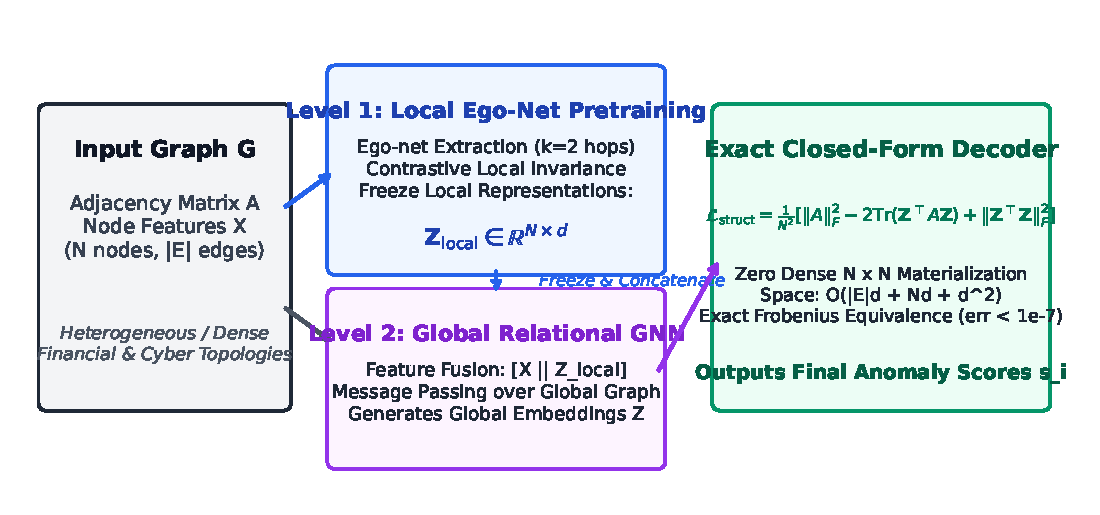
\includegraphics[width=0.92\textwidth]{figures/fig_dlg_architecture.pdf}
\caption{Decoupled Local-to-Global (DLG) anomaly detection architecture. In Level 1, a local GCN feature autoencoder pretrains on full-graph attributes using a finite 2-hop message-passing receptive field (without explicit ego-subgraph induction) and extracts frozen local representation $\mathbf{Z}_{\mathrm{local}}$. In Level 2, the global relational encoder processes the augmented representation $[\mathbf{X} \parallel \mathbf{Z}_{\mathrm{local}}]$ across graph topology $\mathcal{E}$. The attribute decoder reconstructs original attributes $\mathbf{X}$, while the structure decoder computes the unsquashed Gram matrix $\hat{S} = \mathbf{Z} \mathbf{Z}^\top$. Per-node anomaly scores combine Euclidean attribute and structural reconstruction residuals.}
\label{fig:dlg_architecture}
\end{figure}

\subsection{Closed-Form Exact Gram Decoders}
A primary source of memory failure in structural autoencoders (e.g., DOMINANT, DLG-Base, DLG-Aug) is the evaluation of the squared Frobenius reconstruction error against adjacency matrix $A \in \{0, 1\}^{N \times N}$:
\begin{equation}
\mathcal{L}_{\mathrm{struct}} = \frac{1}{N^2} \sum_{i=1}^N \sum_{j=1}^N \left(A_{ij} - \mathbf{z}_i^\top \mathbf{z}_j\right)^2,
\label{eq:dense_loss}
\end{equation}
where $\mathbf{z}_i \in \mathbb{R}^d$ denotes the latent embedding of node $i$. 

In standard implementations, direct computation requires materializing the dense inner product matrix $\mathbf{Z} \mathbf{Z}^\top \in \mathbb{R}^{N \times N}$. For single-precision float32 data, a single contiguous $N \times N$ matrix requires $4 N^2$ bytes, which corresponds to $10.0\,\mathrm{GB}$ ($9.31\,\mathrm{GiB}$) at $N=50,000$ and $160.0\,\mathrm{GB}$ ($149.01\,\mathrm{GiB}$) at $N=200,000$. Materializing two such dense matrices simultaneously (the target adjacency $A$ and the predicted reconstruction $\mathbf{Z} \mathbf{Z}^\top$) requires $8 N^2$ bytes, consuming approximately $20.0\,\mathrm{GB}$ and $320.0\,\mathrm{GB}$ in decimal gigabytes, respectively, before autograd computational graph allocations and workspace overhead. This dense materialization rapidly exhausts GPU device memory.

For unsquashed dot-product decoders (the default setting in PyGOD DOMINANT with \texttt{sigmoid\_s=False}), we expand Equation~\eqref{eq:dense_loss} algebraically:
\begin{align}
\sum_{j=1}^N \left(A_{ij} - \mathbf{z}_i^\top \mathbf{z}_j\right)^2 &= \sum_{j=1}^N A_{ij}^2 - 2 \mathbf{z}_i^\top \sum_{j=1}^N A_{ij} \mathbf{z}_j + \sum_{j=1}^N (\mathbf{z}_i^\top \mathbf{z}_j)^2 \nonumber \\
&= \mathrm{deg}(i) - 2 \mathbf{z}_i^\top \left(A \mathbf{Z}\right)_i + \mathbf{z}_i^\top \left(\mathbf{Z}^\top \mathbf{Z}\right) \mathbf{z}_i,
\label{eq:gram_identity}
\end{align}
where $\mathrm{deg}(i) = \sum_j A_{ij}^2 = \sum_j A_{ij}$ for unweighted binary graphs. Following standard PyGOD semantics (\texttt{double\_recon\_loss}), both inference anomaly scoring and model training optimize the per-node Euclidean $L_2$ row residual norm. Specifically, the per-node structural residual is computed in closed form via Equation~\eqref{eq:gram_identity} without materializing dense $N \times N$ matrices:
\begin{equation}
\mathcal{A}_{\mathrm{struct}, i} = \|A_{i,:} - \hat{A}_{i,:}\|_2 = \sqrt{\max\left(\mathrm{deg}(i) - 2 \mathbf{z}_i^\top (A \mathbf{Z})_i + \mathbf{z}_i^\top (\mathbf{Z}^\top \mathbf{Z}) \mathbf{z}_i, \, 0\right)}.
\label{eq:node_structural_score}
\end{equation}
The composite training loss minimizes the sample mean of the per-node Euclidean residuals:
\begin{equation}
\mathcal{L} = \frac{1}{N} \sum_{i=1}^N \left[ w \|X_{i,:} - \hat{X}_{i,:}\|_2 + (1 - w) \mathcal{A}_{\mathrm{struct}, i} \right],
\label{eq:exact_gram_loss}
\end{equation}
with $w=0.5$. In this formulation, the total structural reconstruction energy prior to the per-node square root corresponds to the Frobenius identity $\frac{1}{N^2}\|A - \mathbf{Z}\mathbf{Z}^\top\|_F^2 = \frac{1}{N^2} [\|A\|_F^2 - 2 \mathrm{Tr}(\mathbf{Z}^\top A \mathbf{Z}) + \|\mathbf{Z}^\top \mathbf{Z}\|_F^2]$, while Equation~\eqref{eq:exact_gram_loss} matches PyGOD's canonical DOMINANT training objective identically down to machine precision ($< 10^{-15}$ relative error in float64) while operating in $\mathcal{O}(N d + |E| d + d^2)$ memory rather than $\mathcal{O}(N^2)$. Controlled unit tests on synthetic directed and undirected graphs ($N=40$) confirmed forward loss, backward gradient, and 10-step Adam trajectory equivalence with PyGOD's dense implementation within floating-point precision.

We emphasize that this exact algebraic reduction strictly requires an unsquashed dot-product decoder. For models such as AnomalyDAE that apply a non-linear sigmoid activation $\sigma(\mathbf{z}_i^\top \mathbf{z}_j)$ to structure reconstruction, the sum cannot be decoupled via Gram matrices in closed form. For AnomalyDAE, we instead implemented a chunked row-block evaluation that computes $B \times N$ cross-reconstructions iteratively ($B=2,048$), reducing peak VRAM from $O(N^2)$ to $O(B N)$ while retaining exact $O(N^2)$ arithmetic.

\section{Experimental Setup and Evaluation Protocol}
\label{sec:experimental_setup}

\subsection{Datasets and Provenance}
We evaluate 13 primary graph datasets spanning native financial ecosystems and standard benchmark graphs, plus one external enterprise cybersecurity network, as summarized in Table~\ref{tab:dataset_properties}.

\begin{table}[htbp]
\centering\fontsize{7.5pt}{8.8pt}\selectfont\setlength{\tabcolsep}{2.5pt}
\caption{Benchmark graph dataset properties, evaluated model-input populations, target label provenance, and evaluation test prevalence. Model-input counts ($N, E, d$) reflect the exact tensors evaluated by all models; upstream raw source graph totals are reported separately. Graph Target Prevalence ($\pi_{\mathrm{graph}} = y_{\mathrm{pos}} / N$) reflects whole-graph label proportions; Evaluated Test Prevalence ($\pi_{\mathrm{test}}$) defines the empirical no-skill AP baseline on the evaluated test split (mean across seeds 42--46).}
\label{tab:dataset_properties}
\begin{tabularx}{\textwidth}{lrrrrr>{\raggedright\arraybackslash}X}\toprule
\textbf{Dataset} & \textbf{Nodes ($N$)} & \textbf{Edges ($E$)} & \textbf{Dim ($d$)} & $\pi_{\mathrm{graph}}$ & $\pi_{\mathrm{test}}$ & \textbf{Target Provenance and Evaluated Population} \\\midrule
\multicolumn{7}{l}{\textit{Native Financial / Blockchain Datasets ($N=5$)}} \\
Elliptic & $46,564$ & $83,188$ & $165$ & $0.0976$ & $0.0976$ & Bitcoin transaction graph; illicit entities \cite{weber2019elliptic}. Evaluated induced graph: 46,564 nodes (raw source: 203,769 nodes). \\
DGraphFin & $1,225,601$ & $746,271$ & $17$ & $0.0127$ & $0.0127$ & FinTech loan user graph; fraudulent defaulters \cite{huang2022dgraph}. Evaluated induced graph: 1,225,601 nodes (raw source: 3,700,550 nodes). \\
Ethereum & $14,385$ & $115,065$ & $8$ & $0.4184$ & $0.4089^*$ & Token-transfer feature-similarity graph; verified phishing/scam contracts \cite{luo2024multichain}. Test split: 2,893 nodes ($40.89\%$ fraud). \\
BSC & $7,481$ & $59,832$ & $8$ & $0.1476$ & $0.1473^*$ & Binance Smart Chain token transfer graph; fraud contracts \cite{luo2024multichain}. Test split: 1,500 nodes ($14.73\%$ fraud). \\
Polygon & $2,303$ & $18,411$ & $8$ & $0.0261$ & $0.0259^*$ & Polygon token transfer graph; verified fraud contracts \cite{luo2024multichain}. Test split: 471 nodes ($2.59\%$ fraud). \\
\midrule
\multicolumn{7}{l}{\textit{Injected Synthetic Benchmarks ($N=8$, including Real Trust Graph with Injected Targets)}} \\
BitcoinOTC & $6,005$ & $7,409$ & $67$ & $0.0300$ & $0.0300$ & SNAP OTC signed trust network \cite{kumar2016edge,snapbitcoinotc}; controlled injected anomaly targets on real graph. Test split: 3,003 nodes. \\
Yelp-Syn & $716,847$ & $14,004,995$ & $300$ & $0.0100$ & $0.0100$ & Social review network; injected structural and contextual anomalies. (PyG/PyGOD evaluated tensor: 716,847 nodes). Test split: 358,424 nodes. \\
Amazon-Syn & $13,752$ & $507,378$ & $767$ & $0.0300$ & $0.0300$ & Co-purchasing graph; injected structural and contextual anomalies. (PyG/PyGOD evaluated tensor: 13,752 nodes). Test split: 6,876 nodes. \\
Reddit-Syn & $232,965$ & $114,869,737$ & $602$ & $0.0200$ & $0.0200$ & Reddit post interaction graph; injected structural anomalies. (PyG/PyGOD evaluated tensor: 232,965 nodes). Test split: 116,483 nodes. \\
Flickr-Syn & $89,250$ & $1,001,494$ & $500$ & $0.0200$ & $0.0200$ & Image sharing network; injected structural anomalies. (PyG/PyGOD evaluated tensor: 89,250 nodes). Test split: 44,625 nodes. \\
Cora-Syn & $2,708$ & $11,276$ & $1433$ & $0.0299$ & $0.0298^*$ & Citation network; injected structural anomalies (PyGOD generator). (PyG/PyGOD evaluated tensor: 2,708 nodes). Test split: 1,354 nodes. \\
CiteSeer-Syn & $3,327$ & $9,914$ & $3703$ & $0.0298$ & $0.0300$ & Citation network; injected structural anomalies (PyGOD generator). (PyG/PyGOD evaluated tensor: 3,327 nodes). Test split: 1,664 nodes. \\
PubMed-Syn & $19,717$ & $93,958$ & $500$ & $0.0300$ & $0.0300$ & Citation network; injected structural anomalies (PyGOD generator). (PyG/PyGOD evaluated tensor: 19,717 nodes). Test split: 9,859 nodes. \\
\midrule
\multicolumn{7}{l}{\textit{External Enterprise Cybersecurity Network ($N=1$)}} \\
LANL-RedTeam & $16,694$ & $323,897$ & $13$ & $0.0180$ & $0.0180$ & Enterprise authentication graph; red-team compromised computers \cite{kent2015cyberdata}. Evaluated destination computers: 16,694 nodes. Test split: 3,338 nodes. \\
\bottomrule
\end{tabularx}
\begin{tablenotes}\footnotesize
\item $^*$ For datasets with seed-dependent evaluation splits (stratified for synthetic benchmarks; seeded random non-stratified 60/20/20 splits for cryptocurrency graphs), $\pi_{\mathrm{test}}$ denotes the empirical mean test-set positive rate across seeds 42--46 (Ethereum: $0.3951$--$0.4307$, mean $0.4089$; BSC: $0.1353$--$0.1600$, mean $0.1473$; Polygon: $0.0149$--$0.0382$, mean $0.0259$; Cora: $0.0295$--$0.0303$, mean $0.0298$).
\end{tablenotes}
\end{table}

\subsection{Evaluation Protocol and Metrics}
All models are evaluated transductively under five random seeds (seeds 42--46). Labels are strictly withheld during training.
\begin{itemize}
    \item \textbf{Average Precision (PR-AUC):} Primary ranking metric, particularly sensitive to low-prevalence imbalances: $\mathrm{AP} = \sum_k (R_k - R_{k-1}) P_k$.
    \item \textbf{ROC-AUC:} Area under the receiver operating characteristic curve, measuring overall discrimination.
    \item \textbf{Alert-Budget Precision and Recall ($\mathbf{P@K}$, $\mathbf{R@K}$):} Evaluated at $K \in \{1\%, 5\%\}$ of total test nodes, measuring practical forensic yield when investigating top-ranked candidates.
    \item \textbf{Evaluation Prevalence Baseline:} The no-skill baseline $\pi_{\mathrm{test}} = |V_{\mathrm{test}}^+| / |V_{\mathrm{test}}|$, against which AP gains must be judged.
    \item \textbf{Deterministic Split Identity:} All detectors on a given dataset and seed are evaluated on the exact same test node indices and labels. All detectors evaluate identical test node subsets; on DGraphFin, while serialized metadata formats differ between boolean masks and index arrays, both represent the exact same 183,840-node official test split ($2{,}326$ positives, $\pi_{\mathrm{test}} = 0.0127$).
\end{itemize}

\subsection{Friedman Hypothesis Testing and Permutation Design}
To assess statistical significance across multiple datasets without assuming normal distributions, we employ the Friedman non-parametric test. Let $r_i^j$ denote the rank of detector $j \in \{1, \dots, k\}$ on dataset block $i \in \{1, \dots, n\}$. The Friedman statistic $Q$ is computed with tie corrections:
\begin{equation}
Q = \frac{\frac{12}{n k (k+1)} \sum_{j=1}^k R_j^2 - 3 n (k+1)}{1 - \frac{\sum T_i}{n(k^3 - k)}},
\label{eq:friedman_q}
\end{equation}
where $R_j = \sum_{i=1}^n r_i^j$ is the sum of ranks for model $j$. 

While $Q$ converges asymptotically to $\chi^2_{k-1}$ as $n \to \infty$, benchmark suites typically have small sample sizes ($n \in \{6, 8, 13\}$). Under small $n$, the continuous $\chi^2$ approximation tends to be conservative. We therefore compute exact Monte Carlo within-block permutation $p$-values: within each dataset row, the model ranks are permuted randomly across $B=1,000,000$ replications (pinned seed 20261024), computing the empirical tail probability $p = (b + 1) / (B + 1)$ where $b$ is the number of permutations yielding a statistic greater than or equal to $Q_{\mathrm{obs}}$. For pairwise comparisons against DLG-Aug, we report two-sided Wilcoxon signed-rank tests adjusted via the Holm step-down procedure \cite{holm1979}. We note that for within-dataset comparisons across $N_{\mathrm{seeds}} = 5$, the minimum achievable two-sided Wilcoxon signed-rank $p$-value is $2^{-(5-1)} = 0.0625$ when all five differences share the same nonzero sign. Consequently, no single dataset comparison can attain conventional $\alpha = 0.05$ significance under five seeds alone; statistical hypothesis testing is therefore evaluated across the benchmark suite via the Friedman permutation framework.

To quantify overall rank effect sizes across evaluation views, we compute tie-corrected Kendall's coefficient of concordance $W = Q / [n (k - 1)]$. Under View S1 (seven models on five complete-case datasets), $W=0.780$ indicates strong inter-dataset ranking agreement ($Q=23.40, p < 0.001$). Under View S2 (five models across all 13 primary datasets), $W=0.457$ reflects moderate concordance ($Q=23.75, p = 0.0001$). Domain-specific stratification reveals pronounced divergence: on the mixed-label financial and blockchain view (View S3, $n=6$, comprising five external fraud-label graphs plus BitcoinOTC with canonical injected node anomaly labels on a real trust network), concordance is weak ($W=0.256$), where DLG-Aug attains the top mean rank ($1.83$), whereas on pure synthetic benchmark graphs (View S4, $n=7$), concordance is strong ($W=0.780$) with DLG-Base (mean rank $1.86$) and DOMINANT ($2.00$) dominating.

\section{Results and Empirical Analysis}
\label{sec:results}

\subsection{Evaluated Population and Hardware Support Feasibility}
Figure~\ref{fig:support_matrix} details the execution feasibility across all 14 datasets and seven detector configurations.

\begin{figure}[htbp]
\centering
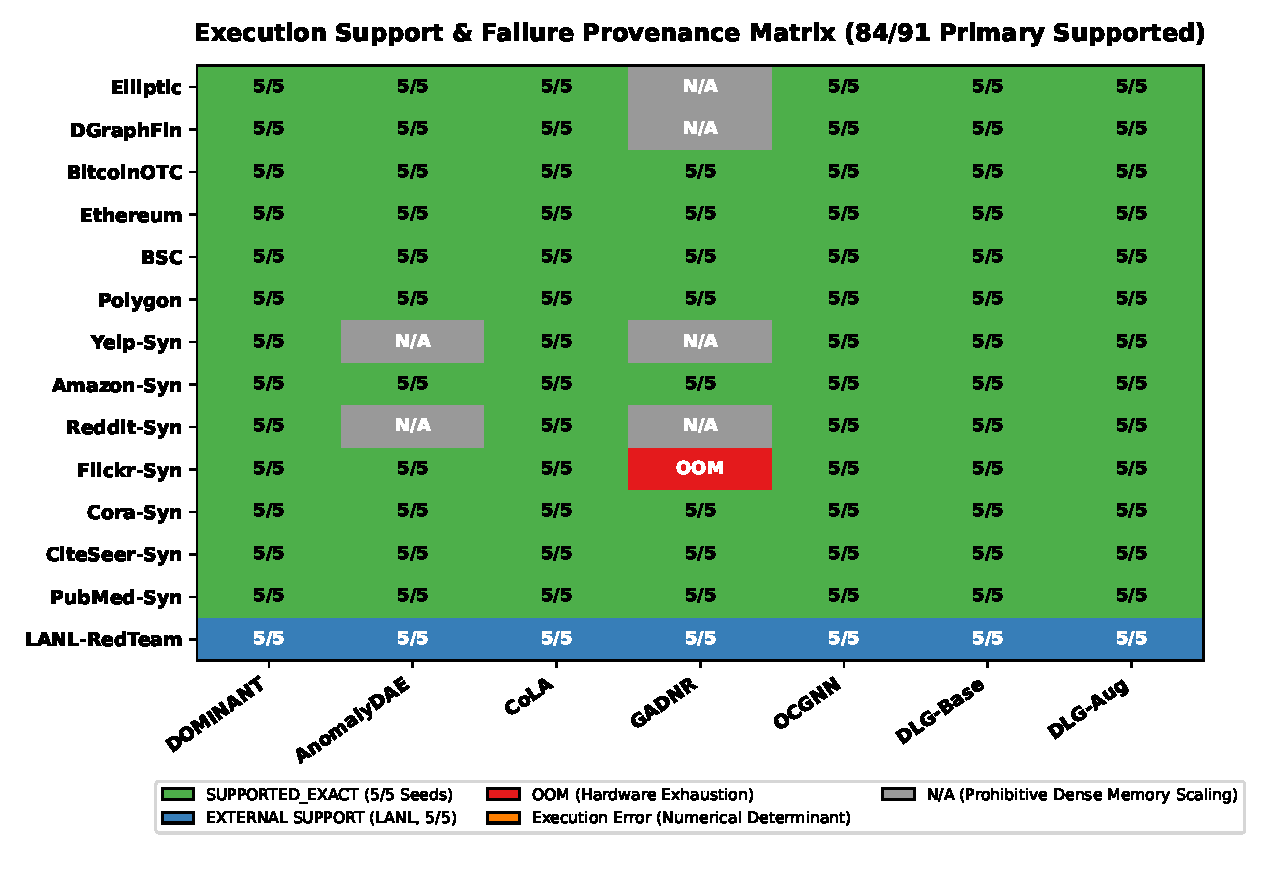
\includegraphics[width=0.88\textwidth]{figures/fig_support_matrix.pdf}
\caption{Hardware support feasibility and failure provenance matrix across 14 graph datasets and seven models in mixed environments (84 of 91 primary pairs fully supported across all five seeds). Cell annotations and shading distinguish exact complete primary support (\texttt{5/5}), external benchmark support on LANL-RedTeam (\texttt{Ext}), execution failure without an approved raw run (four GADNR pairs on Elliptic, DGraphFin, Yelp-Syn, and Reddit-Syn), and out-of-memory hardware exhaustion (one historical 8-GB legacy CUDA OOM for GADNR on Flickr-Syn, and two 24-GB full-encoder-forward CUDA OOMs for AnomalyDAE on Yelp-Syn and Reddit-Syn).}
\label{fig:support_matrix}
\end{figure}

Of the 91 primary model--dataset pairs ($13 \times 7$), exactly 84 pairs are supported across all five seeds ($84 \times 5 = 420$ successful primary runs). GADNR is unsupported on five graphs across two distinct failure modes: four pairs (Elliptic, DGraphFin, Yelp-Syn, and Reddit-Syn) suffered historical numerical covariance determinant failures without approved raw runs, while one pair (Flickr-Syn) encountered memory exhaustion on a legacy 8-GB environment. AnomalyDAE is unsupported on two graphs (Yelp-Syn and Reddit-Syn) due to out-of-memory exceptions during the full-graph encoder forward pass on a 24-GB GPU (yielding seven unsupported primary pairs in total). In contrast, the exact Gram formulations developed in Section~\ref{sec:models} allow DOMINANT, DLG-Base, and DLG-Aug to complete all runs successfully without memory overflow, even on the 1.2-million-node DGraphFin graph.

\subsection{Predictive Quality vs.\ Evaluation Prevalence and Alert Budgets}
Table~\ref{tab:pr_auc_main} reports the Average Precision (PR-AUC) performance of all seven detectors alongside the evaluation prevalence baseline.

\begin{table}[htbp]
\centering\footnotesize\setlength{\tabcolsep}{1.8pt}
\caption{Average Precision (PR-AUC; mean across five seeds). Evaluated test prevalence ($\pi_{\mathrm{test}}$) defines the empirical no-skill random-ranking baseline on the evaluated test split. Unsupported cells are denoted as N/A.}
\label{tab:pr_auc_main}
\begin{tabular*}{\textwidth}{@{\extracolsep{\fill}}lrrrrrrrr}\toprule
\textbf{Dataset} & $\pi_{\mathrm{test}}$ & \textbf{DOMINANT} & \textbf{AnomalyDAE} & \textbf{CoLA} & \textbf{GADNR} & \textbf{OCGNN} & \textbf{DLG-Base} & \textbf{DLG-Aug} \\\midrule
Elliptic & $0.0976$ & 0.0682 & 0.0538 & 0.0947 & N/A & 0.0667 & 0.0687 & \textbf{0.1037} \\
DGraphFin & $0.0127$ & 0.0102 & 0.0119 & 0.0127 & N/A & 0.0126 & 0.0101 & \textbf{0.0134} \\
BitcoinOTC & $0.0300$ & \textbf{0.8810} & 0.7948 & 0.4936 & 0.8125 & 0.0290 & 0.8274 & 0.8211 \\
Ethereum & $0.4089$ & 0.3971 & 0.3986 & 0.3648 & 0.3976 & \textbf{0.4996} & 0.4106 & 0.4359 \\
BSC & $0.1473$ & 0.2299 & \textbf{0.3609} & 0.1252 & 0.1561 & 0.1615 & 0.3390 & 0.3411 \\
Polygon & $0.0259$ & 0.1071 & \textbf{0.1878} & 0.0232 & 0.0260 & 0.0700 & 0.0854 & 0.0731 \\
Yelp-Syn & $0.0100$ & 0.0749 & N/A & 0.0174 & N/A & 0.0069 & 0.0826 & \textbf{0.0832} \\
Amazon-Syn & $0.0300$ & 0.1301 & \textbf{0.2734} & 0.0989 & 0.0338 & 0.0249 & 0.1245 & 0.1302 \\
Reddit-Syn & $0.0200$ & \textbf{0.4069} & N/A & 0.1606 & N/A & 0.0205 & 0.4044 & 0.3388 \\
Flickr-Syn & $0.0200$ & 0.4610 & \textbf{0.4761} & 0.0447 & N/A & 0.0247 & 0.4569 & 0.4599 \\
Cora-Syn & $0.0298$ & 0.4740 & 0.4494 & 0.0299 & 0.0951 & 0.0302 & \textbf{0.4758} & 0.4720 \\
CiteSeer-Syn & $0.0300$ & 0.5989 & 0.5507 & 0.0304 & 0.3662 & 0.0301 & \textbf{0.6004} & 0.5992 \\
PubMed-Syn & $0.0300$ & 0.1607 & \textbf{0.6837} & 0.0705 & 0.1014 & 0.0300 & 0.1623 & 0.1605 \\\midrule
LANL-RedTeam & $0.0180$ & 0.1348 & 0.0450 & 0.0200 & \textbf{0.1806} & 0.0454 & 0.1367 & 0.1114 \\\bottomrule
\end{tabular*}
\begin{tablenotes}\footnotesize
\item Note: For datasets with seed-dependent evaluation splits (stratified for synthetic graphs; seeded random non-stratified 60/20/20 splits for cryptocurrency graphs), $\pi_{\mathrm{test}}$ reports the empirical mean test positive rate across seeds 42--46.
\end{tablenotes}
\end{table}

\textbf{Interpretation of Prevalence Baselines and Comparator Superiority:}
\begin{enumerate}
    \item On the Elliptic dataset, DLG-Aug is the only model achieving AP higher than the test prevalence ($0.1037 > 0.0976$; lift $\approx 1.063\times$), whereas DOMINANT ($0.0682$), AnomalyDAE ($0.0538$), and DLG-Base ($0.0687$) fall below random baseline precision.
    \item On DGraphFin, all detectors perform near the empirical no-skill prevalence baseline ($\pi_{\mathrm{test}} = 0.0127$), with DLG-Aug ($0.0134$) and CoLA ($0.0127$) performing essentially at or slightly above prevalence (lift $\approx 1.055\times$), while other baselines fall slightly below.
    \item On the three cryptocurrency networks, established comparators outperform DLG-Aug: OCGNN achieves the highest AP on Ethereum ($0.4996$ vs.\ Aug $0.4359$, both exceeding the $0.4089$ test prevalence), while AnomalyDAE leads on BSC ($0.3609$ vs.\ Aug $0.3411$) and Polygon ($0.1878$ vs.\ Aug $0.0731$). Thus, \textit{at least one established comparator exceeds DLG-Aug in mean AP on each of the three blockchain datasets.}
\end{enumerate}

Table~\ref{tab:alert_budget} evaluates operational alert budgets on the three cryptocurrency graphs, measuring Precision@1\%, Recall@1\%, Precision@5\%, and Recall@5\%.

\begin{table}[htbp]
\centering\small\setlength{\tabcolsep}{3.5pt}
\caption{Operational Alert-Budget Performance across Cryptocurrency Benchmarks (mean across five seeds). Metrics denote precision and recall when auditing the top-1\% and top-5\% highest-scoring nodes. On Polygon ($N_{\mathrm{test}}=471, K@1\%=5, M_{\mathrm{test}} \in [7, 18]$), single-count true positive detections alter Precision@1\% by $0.200$; these low-budget results represent exploratory evidence under discrete sample variance.}
\label{tab:alert_budget}
\begin{tabularx}{\textwidth}{llrrrrrrr}\toprule
\textbf{Dataset} & \textbf{Metric} & \textbf{DOMINANT} & \textbf{AnomalyDAE} & \textbf{CoLA} & \textbf{GADNR} & \textbf{OCGNN} & \textbf{DLG-Base} & \textbf{DLG-Aug} \\\midrule
\multirow{4}{*}{Ethereum} & $P@1\%$ & $\mathbf{0.4897}$ & $0.2621$ & $0.3034$ & $0.4621$ & $0.3931$ & $0.4690$ & $0.4621$ \\
 & $R@1\%$ & $\mathbf{0.0121}$ & $0.0064$ & $0.0074$ & $0.0113$ & $0.0098$ & $0.0115$ & $0.0114$ \\
 & $P@5\%$ & $\mathbf{0.5145}$ & $0.3117$ & $0.3779$ & $0.4110$ & $0.5090$ & $0.4800$ & $0.5007$ \\
 & $R@5\%$ & $0.0631$ & $0.0381$ & $0.0463$ & $0.0503$ & $\mathbf{0.0632}$ & $0.0591$ & $0.0620$ \\
\midrule
\multirow{4}{*}{BSC} & $P@1\%$ & $0.1867$ & $\mathbf{0.3867}$ & $0.0533$ & $0.1733$ & $0.2133$ & $0.2800$ & $0.3067$ \\
 & $R@1\%$ & $0.0126$ & $\mathbf{0.0261}$ & $0.0036$ & $0.0116$ & $0.0145$ & $0.0187$ & $0.0207$ \\
 & $P@5\%$ & $0.2827$ & $\mathbf{0.4507}$ & $0.0720$ & $0.1653$ & $0.1600$ & $0.4133$ & $0.4133$ \\
 & $R@5\%$ & $0.0959$ & $\mathbf{0.1527}$ & $0.0242$ & $0.0556$ & $0.0545$ & $0.1397$ & $0.1402$ \\
\midrule
\multirow{4}{*}{Polygon} & $P@1\%$ & $0.2400$ & $\mathbf{0.3600}$ & $0.0000$ & $0.0000$ & $0.0400$ & $0.0400$ & $0.0800$ \\
 & $R@1\%$ & $0.1114$ & $\mathbf{0.1566}$ & $0.0000$ & $0.0000$ & $0.0286$ & $0.0111$ & $0.0236$ \\
 & $P@5\%$ & $0.1083$ & $\mathbf{0.1500}$ & $0.0000$ & $0.0000$ & $0.0583$ & $0.1000$ & $0.0833$ \\
 & $R@5\%$ & $0.2102$ & $\mathbf{0.2964}$ & $0.0000$ & $0.0000$ & $0.1323$ & $0.1984$ & $0.1651$ \\
\bottomrule
\end{tabularx}
\end{table}

\subsection{Conditional Utility Analysis and Delta Distribution}
Figure~\ref{fig:conditional_delta} and Table~\ref{tab:conditional_delta} illustrate the signed performance differential ($\Delta\mathrm{AP} = \mathrm{AP}_{\mathrm{Aug}} - \mathrm{AP}_{\mathrm{Base}}$) across all 14 evaluated benchmarks.

\begin{figure}[htbp]
\centering
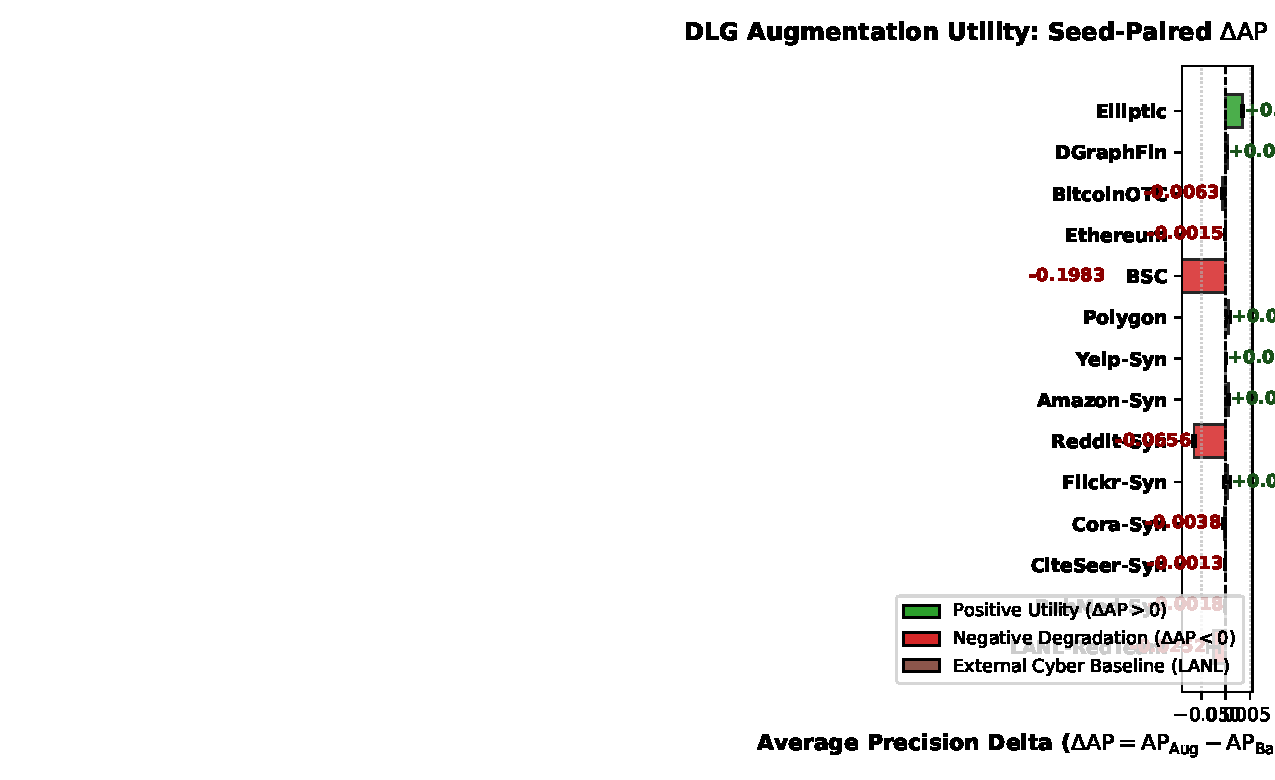
\includegraphics[width=0.88\textwidth]{figures/fig_conditional_delta.pdf}
\caption{Conditional AP delta ($\Delta\mathrm{AP} = \mathrm{AP}_{\mathrm{Aug}} - \mathrm{AP}_{\mathrm{Base}}$) across all 13 primary datasets plus external LANL-RedTeam (with paired seed-level standard error bars, $n=5$ seeds). Localized representation augmentation yields positive observed mean paired differences on Elliptic ($+0.0350$) and Ethereum ($+0.0253 \pm 0.0144$), near-zero observed difference on BSC ($+0.0021 \pm 0.0103$), but incurs observed performance degradation on Polygon ($-0.0124 \pm 0.0054$), Reddit-Syn ($-0.0656 \pm 0.0031$), and LANL-RedTeam ($-0.0252 \pm 0.0126$).}
\label{fig:conditional_delta}
\end{figure}

\begin{table}[htbp]
\centering\fontsize{7.6pt}{8.9pt}\selectfont\setlength{\tabcolsep}{4pt}\renewcommand{\arraystretch}{0.92}
\renewcommand{\arraystretch}{0.92}
\caption{Observed Average Precision performance of DLG-Base versus DLG-Aug across all 14 evaluated datasets (13 primary graphs plus external LANL-RedTeam). Results report mean AP, observed seed-paired differences ($\Delta\mathrm{AP} = \mathrm{AP}_{\mathrm{Aug}} - \mathrm{AP}_{\mathrm{Base}}$), and paired standard errors ($n=5$ random seeds). Localized structural augmentation exhibits positive observed differences on certain transaction graphs but performance trade-offs on dense social networks and cyber authentication graphs. Relative percentage differences ($(\mathrm{AP}_{\mathrm{Aug}} - \mathrm{AP}_{\mathrm{Base}})/\mathrm{AP}_{\mathrm{Base}}$) are reported in notes for reference alongside absolute differences.}
\label{tab:conditional_delta}
\begin{tabularx}{\textwidth}{lrrrr>{\raggedright\arraybackslash}X}\toprule
\textbf{Dataset} & \textbf{DLG-Base (AP)} & \textbf{DLG-Aug (AP)} & $\mathbf{\Delta\mathrm{AP}}$ & \textbf{Paired SE} & \textbf{Operational Characterization} \\\midrule
Elliptic & $0.0687$ & $0.1037$ & $\mathbf{+0.0350}$ & $\pm 0.0022$ & \textbf{Observed Gain} ($\Delta\mathrm{AP} = +0.0350$; lift over prevalence $\approx 1.063\times$; relative gain $+50.97\%$ over Base); positive paired difference observed. \\
DGraphFin & $0.0101$ & $0.0134$ & $+0.0034$ & $\pm 0.0008$ & \textbf{Slight Gain} ($\Delta\mathrm{AP} = +0.0034$; lift $\approx 1.055\times$); performs near no-skill prevalence; exact full-graph execution supported. \\
BitcoinOTC & $0.8274$ & $0.8211$ & $-0.0063$ & $\pm 0.0033$ & \textbf{Slight Loss} ($-0.77\%$ rel.); high baseline precision ($0.827$) retains competitive performance. \\
Ethereum & $0.4106$ & $0.4359$ & $\mathbf{+0.0253}$ & $\pm 0.0144$ & \textbf{Gain} ($+6.15\%$ rel.); DLG-Aug has higher mean AP in this constructed similarity-graph evaluation. \\
BSC & $0.3390$ & $0.3411$ & $+0.0021$ & $\pm 0.0103$ & \textbf{Marginal Gain} ($+0.61\%$ rel.); slight positive mean difference on BSC token transfers. \\
Polygon & $0.0854$ & $0.0731$ & $-0.0124$ & $\pm 0.0054$ & \textbf{Loss} ($-14.48\%$ rel.); negative $\Delta\mathrm{AP}$ observed in this similarity-graph evaluation. \\
Yelp-Syn & $0.0826$ & $0.0832$ & $+0.0007$ & $\pm 0.0015$ & Stable / marginal gain on injected contextual/structural anomaly patterns. \\
Amazon-Syn & $0.1245$ & $0.1302$ & $+0.0057$ & $\pm 0.0016$ & Stable / marginal gain on injected contextual/structural anomaly patterns. \\
Reddit-Syn & $0.4044$ & $0.3388$ & $\mathbf{-0.0656}$ & $\pm 0.0031$ & \textbf{Substantial Loss} ($-16.22\%$ rel.); negative delta observed on dense social interaction graph. \\
Flickr-Syn & $0.4569$ & $0.4599$ & $+0.0030$ & $\pm 0.0076$ & Stable / marginal gain on injected contextual/structural anomaly patterns. \\
Cora-Syn & $0.4758$ & $0.4720$ & $-0.0038$ & $\pm 0.0031$ & Stable observed performance on citation graphs. \\
CiteSeer-Syn & $0.6004$ & $0.5992$ & $-0.0013$ & $\pm 0.0014$ & Stable observed performance on citation graphs. \\
PubMed-Syn & $0.1623$ & $0.1605$ & $-0.0018$ & $\pm 0.0003$ & Stable observed performance on citation graphs. \\
LANL-RedTeam$^{\dagger}$ & $0.1367$ & $0.1114$ & $-0.0252$ & $\pm 0.0126$ & \textbf{External Loss} ($-18.47\%$ rel.); negative $\Delta\mathrm{AP}$ observed on cyber authentication event graph. \\
\bottomrule
\end{tabularx}
\begin{tablenotes}\footnotesize
\item $^{\dagger}$ LANL-RedTeam is an external enterprise cybersecurity network evaluated under identical protocol but reported as single-graph descriptive evidence.
\end{tablenotes}
\end{table}


The empirical evidence does not support a universal benefit from pretrained local-feature augmentation under the studied conditions. While DLG-Aug yields positive observed mean paired differences on transaction graphs like Elliptic ($\Delta\mathrm{AP} = +0.0350$) and Ethereum ($\Delta\mathrm{AP} = +0.0253$), it exhibits lower performance on Reddit-Syn ($\Delta\mathrm{AP} = -0.0656$) and LANL-RedTeam ($\Delta\mathrm{AP} = -0.0252$).

\subsection{Cross-Dataset Omnibus Evaluation and Permutation Statistics}
Table~\ref{tab:friedman_stats} summarizes the Friedman omnibus test results across four evaluation views (S1--S4).

\begin{table}[htbp]
\centering\footnotesize\setlength{\tabcolsep}{2.5pt}
\caption{Complete-case Friedman non-parametric test statistics and $p$-values across four evaluation views under $1{,}000{,}000$ Monte Carlo within-block permutations (seed 20261024). $n$ and $k$ denote the number of dataset blocks and comparative models, respectively; $Q$ is the Friedman test statistic; $b$ is the permutation exceedance count. Exact tail probabilities are computed as $p = (b+1)/(B+1)$ alongside asymptotic $\chi^2$ references.}
\label{tab:friedman_stats}
\begin{tabularx}{\textwidth}{lcccccc>{\raggedright\arraybackslash}X}\toprule
\textbf{View} & \textbf{$n$} & \textbf{$k$} & \textbf{Stat ($Q$)} & $\chi^2\ p$ & \textbf{Exceed. ($b$)} & \textbf{1M MC $p \pm \text{SE}$} & \textbf{Statistical Inference} \\\midrule
\textbf{S1} (8 DS, 7 M) & 8 & 7 & $29.0357$ & $5.99e-05$ & 3 & $4.00e-06 \pm 2.0e-06$ & \textbf{Significant} ($p < 0.05$); reject null of equal detector ranking. \\
\textbf{S2} (13 DS, 5 M) & 13 & 5 & $23.7538$ & $8.95e-05$ & 20 & $2.10e-05 \pm 4.6e-06$ & \textbf{Significant} ($p < 0.05$); reject null of equal detector ranking. \\
\textbf{S3} (6 DS, 5 M) & 6 & 5 & $6.1333$ & $1.89e-01$ & 192,107 & $1.92e-01 \pm 3.9e-04$ & \textit{Non-significant} ($p = 0.1921$); no statistically significant difference in detector ranking observed (not evidence of ranking equivalence). \\
\textbf{S4} (7 DS, 5 M) & 7 & 5 & $21.8286$ & $2.17e-04$ & 0 & $1.00e-06 \pm 1.0e-06$ & \textbf{Significant} ($p < 0.05$); zero exceedances ($b=0$) yields add-one estimate $p_{\mathrm{MC}} \approx 1.0 \times 10^{-6}$ with one-sided 95\% upper confidence bound $\approx 3.0 \times 10^{-6}$; reject null. \\
\bottomrule
\end{tabularx}
\end{table}

\textbf{Statistical Explanation of Asymptotic vs.\ Permutation Discrepancies:}
The asymptotic $\chi^2$ approximation and the within-block Monte Carlo permutation test yielded different tail probabilities across the evaluation views. We report the permutation design, random seed (seed 20261024), replicate count ($B=1{,}000{,}000$), exceedance counts, and Monte Carlo uncertainty alongside the asymptotic reference values:
\begin{itemize}
    \item In the tested finite complete-case configurations ($n \in \{6, 7, 8\}$ as well as $n=13$ in S2), the discrete permutation space $\prod_{i=1}^n (k!)$ exhibits distinct tail behavior compared to the continuous $\chi^2_{k-1}$ distribution. Ranking configurations therefore yield smaller tail probabilities under the exact discrete within-block permutation null than under the asymptotic $\chi^2$ limit in these observed settings.
    \item At $B=1{,}000{,}000$, we observe exactly 3 exceedances for S1 ($p = 4.0 \times 10^{-6}$), 20 for S2 ($p = 2.1 \times 10^{-5}$), and 0 for S4. For S4, observing $b=0$ yields the standard add-one Monte Carlo estimate $p_{\mathrm{MC}} = (0+1)/(1{,}000{,}000+1) \approx 1.0 \times 10^{-6}$, with an approximate one-sided 95\% upper confidence bound on the unknown tail probability of $-\ln(0.05)/B \approx 3.0 \times 10^{-6}$ (rather than a deterministic zero-tail claim), confirming that the frozen MC results capture the empirical tail probability.
\end{itemize}

Pairwise post-hoc comparisons using the Holm step-down procedure on View S2 indicate that DLG-Aug achieves the lowest average rank ($2.0000$), followed closely by DOMINANT ($2.3846$) and DLG-Base ($2.5385$). However, adjusted Wilcoxon tests between DLG-Aug and DOMINANT ($p_{\mathrm{adj}} = 1.0000$) and DLG-Base ($p_{\mathrm{adj}} = 1.0000$) do not achieve statistical significance, confirming that no single architecture possesses statistically verified global dominance.

\section{Execution, Memory, and Computational Complexity}
\label{sec:execution_complexity}
To illustrate the practical computational scaling of the evaluated methods, Table~\ref{tab:complexity_comparison} compares theoretical asymptotic complexity against illustrative peak GPU memory materialization profiles on an NVIDIA GeForce RTX 3090 24 GB GPU platform.

\begin{table}[htbp]
\centering\footnotesize\setlength{\tabcolsep}{3pt}
\caption{Theoretical computational complexity and illustrative peak memory materialization profiles for graph anomaly detector architectures. Memory entries indicate estimated peak allocated GPU memory scaling profiles under PyTorch (batch size $B=2{,}048$ for row-blocked formulations) on an RTX 3090 24GB platform; values serve as illustrative architectural scaling profiles rather than hardware-invariant empirical benchmarks. For dense formulations on Reddit-Syn ($N=232,965$), a single float32 dense matrix requires $4 N^2 \approx 217\,\mathrm{GB}$ decimal, mathematically exceeding 24GB GPU capacity. Full AnomalyDAE remains unsupported on Reddit-Syn in our benchmark due to dense structure encoder memory limits. $^\dagger$Theoretical structural-stage memory estimate under row blocking ($B=2{,}048$); its full-graph dual-encoder forward pass incurs CUDA OOM on 24GB hardware. $^\ddagger$GADNR on Reddit-Syn, Elliptic, DGraphFin, and Yelp-Syn is categorized in the benchmark registry as execution failure without an approved raw run (\texttt{NO\_APPROVED\_RAW\_RUN}); post-hoc synthetic diagnostics illustrate how rank-deficient neighborhood covariance matrices induce Cholesky determinant breakdown during Gaussian density estimation. On Flickr-Syn, GADNR encountered historical CUDA OOM on an 8\,GB legacy GPU platform.}
\label{tab:complexity_comparison}
\begin{tabularx}{\textwidth}{lXXrr}\toprule
\textbf{Model} & \textbf{Time Complexity} & \textbf{Space Complexity} & \textbf{Profile (Cora)} & \textbf{Profile (Reddit)} \\\midrule
DOMINANT (Dense PyGOD) & $\mathcal{O}(L |E| d + N^2 d)$ & $\mathcal{O}(N^2 + N d)$ & $\approx 1.2\,\mathrm{GB}$ & $\mathrm{OOM}\ (>24\,\mathrm{GB})$ \\
DOMINANT (Exact Gram) & $\mathcal{O}(L |E| d + N d^2)$ & $\mathcal{O}(|E| d + N d + d^2)$ & $\approx 0.4\,\mathrm{GB}$ & $\approx 4.8\,\mathrm{GB}$ \\
AnomalyDAE (Dense) & $\mathcal{O}(L |E| d + N^2 d)$ & $\mathcal{O}(N^2 + N d)$ & $\approx 1.9\,\mathrm{GB}$ & $\mathrm{OOM}\ (>24\,\mathrm{GB})$ \\
AnomalyDAE (Row-Block)$^\dagger$ & $\mathcal{O}(L |E| d + N^2 d)$ & $\mathcal{O}(B N + N d)$ & $\approx 0.7\,\mathrm{GB}$ & $\approx 7.1\,\mathrm{GB}^\dagger$ \\
CoLA & $\mathcal{O}(S K |E_{\mathrm{sub}}| d)$ & $\mathcal{O}(S K N_{\mathrm{sub}} d)$ & $\approx 0.8\,\mathrm{GB}$ & $\approx 5.9\,\mathrm{GB}$ \\
GADNR & $\mathcal{O}(L |E| d + N K d^2)$ & $\mathcal{O}(|E| d + N K d)$ & $\approx 1.5\,\mathrm{GB}$ & $\mathrm{Unsup.}^\ddagger$ \\
OCGNN & $\mathcal{O}(L |E| d + N d)$ & $\mathcal{O}(|E| d + N d)$ & $\approx 0.3\,\mathrm{GB}$ & $\approx 2.5\,\mathrm{GB}$ \\
DLG-Base (Exact Gram) & $\mathcal{O}(L |E| d + N d^2)$ & $\mathcal{O}(|E| d + N d + d^2)$ & $\approx 0.4\,\mathrm{GB}$ & $\approx 4.9\,\mathrm{GB}$ \\
DLG-Aug (Exact Gram) & $\mathcal{O}((L_{\mathrm{loc}} + L_{\mathrm{glob}}) |E| d)$ & $\mathcal{O}(|E| d + N d + d^2)$ & $\approx 0.5\,\mathrm{GB}$ & $\approx 5.5\,\mathrm{GB}$ \\\bottomrule
\end{tabularx}
\end{table}

The closed-form Gram formulation reduces the asymptotic space complexity of DOMINANT and DLG models from quadratic $\mathcal{O}(N^2)$ to linear in edge density $\mathcal{O}(|E| d + N d)$. On Reddit-Syn ($N=232,965, |E|=114.9\,\mathrm{M}$ directed edges), a single dense float32 adjacency or kernel matrix mathematically requires $4 N^2 \approx 217\,\mathrm{GB}$ of memory (and $6.0\,\mathrm{TB}$ on DGraphFin with $N=1,225,601$), mathematically exceeding physical 24-GB GPU capacity without profiler invocation. The exact Gram decoder enables full-graph training within an illustrative $\approx 5.5\,\mathrm{GB}$ memory profile. We explicitly emphasize that here exact full-graph evaluation designates the entire evaluated induced graph ($N=46,564$ on Elliptic, $N=1,225,601$ on DGraphFin) without neighborhood mini-batch sampling, rather than unclassified or unlinked upstream nodes. Importantly, while row-blocked AnomalyDAE alleviates intermediate reconstruction memory ($\mathcal{O}(B N)$), it retains $\mathcal{O}(N^2)$ arithmetic operations, and its full-graph encoder forward pass still incurs CUDA out-of-memory errors on 24GB hardware, keeping it unsupported in our benchmark.

\section{Discussion: Practical Anomaly-Detection Deployment Guide}
\label{sec:discussion}

\subsection{Practitioner Decision Matrix}
Based on our multi-dataset evaluation, Table~\ref{tab:decision_matrix} presents an operational decision matrix serving as conditional starting points for practitioners deploying unsupervised GAD in financial and cyber domains.

\begin{table}[htbp]
\centering\fontsize{7.2pt}{8.5pt}\selectfont\setlength{\tabcolsep}{2.5pt}
\caption{Practitioner decision matrix providing evidence-calibrated conditional starting points under operational constraints. Computational feasibility is strictly distinguished from predictive precision. Evidence coverage indicates the number of verified datasets ($n$) supporting each regime. On low-prevalence large-scale graphs, full-graph execution support does not imply effective fraud ranking accuracy.}
\label{tab:decision_matrix}
\begin{tabularx}{\textwidth}{>{\raggedright\arraybackslash}p{0.18\textwidth}>{\raggedright\arraybackslash}p{0.20\textwidth}>{\raggedright\arraybackslash}Xc>{\raggedright\arraybackslash}p{0.24\textwidth}}\toprule
\textbf{Regime / Constraint} & \textbf{Supported Starting Point} & \textbf{Predictive Evidence vs.\ Prevalence} & $\mathbf{n}$ & \textbf{Operational Caveat / Unsupported Path} \\\midrule
Transaction networks with high class imbalance (fraud $\approx 9.76\%$; e.g., Elliptic) & \textbf{DLG-Aug} & Surpasses evaluation prevalence ($0.1037 > \pi_{\mathrm{test}}=0.0976$; $\Delta\mathrm{AP}=+0.0350$) & 1 & CoLA ($0.0947$) and Base ($0.0687$) perform below prevalence; GADNR unsupported (execution failure). \\
Large-scale graphs ($N > 10^6$, constrained memory; e.g., DGraphFin) & \textbf{DLG-Base / DOMINANT} with Exact Gram decoder & Full-graph execution supported; predictive AP near no-skill prevalence ($0.0101$--$0.0102$ vs $\pi_{\mathrm{test}}=0.0127$) & 1 & Supported starting point for execution, but does not provide high-precision fraud detection; GADNR unsupported. \\
Dense interaction graphs ($E > 10^8$; e.g., Reddit-Syn) & \textbf{DOMINANT / DLG-Base} & Lead predictive AP ($0.4069$ and $0.4044$ vs $\pi_{\mathrm{test}}=0.0200$) & 1 & DLG-Aug exhibits performance loss ($\Delta\mathrm{AP}=-0.0656$); AnomalyDAE unsupported in 24GB matrix (encoder OOM). \\
Strict alert budgets ($P@1\%$ AML triage; Ethereum, BSC, Polygon) & \textbf{AnomalyDAE} (leads BSC/Polygon); \textbf{DOMINANT} (leads ETH); \textbf{DLG-Aug} (competitive across all 3) & Verified across 105 runs on 3 chains; $P@1\%$ reaches $0.490$ (ETH), $0.387$ (BSC), $0.360$ (Polygon) & 3 & Polygon $K@1\%=5$ ($M_{\mathrm{test}} \in [7, 18]$) is exploratory/unstable ($\Delta P = 0.20$ per TP); non-stratified random test splits. \\
Enterprise authentication event logs (e.g., LANL-RedTeam) & \textbf{GADNR} (leads AP $0.1806$); \textbf{DLG-Base} ($0.1367$) & Descriptive external validation ($0.1806$ vs $\pi_{\mathrm{test}}=0.0180$) & 1 & Single-graph exploratory evidence; DLG-Aug underperforms Base ($\Delta\mathrm{AP}=-0.0252$); pipeline threshold provenance. \\\bottomrule
\end{tabularx}
\end{table}

\subsection{Limitations and Boundary Conditions}
We explicitly delineate the scientific boundaries of this study:
\begin{enumerate}
    \item \textbf{Synthetic Target Injection and Single Seed Injection:} Eight of the 13 primary graphs rely on synthetic anomaly injection (including BitcoinOTC), generated under a single fixed injection seed; synthetic targets may not capture evolving adversarial evasion.
    \item \textbf{Static vs.\ Dynamic Formulations:} Although cryptocurrency transactions and authentication logs occur continuously over time, our benchmark evaluates frozen static projections to ensure comparability across standard GAD architectures. Dynamic graph models and continuous-time temporal architectures (e.g., TGN \cite{rossi2020tgn}, JODIE \cite{kumar2019jodie}, TGAT \cite{xu2020tgat}, EvolveGCN \cite{pareja2020evolvegcn}, DyRep \cite{trivedi2019dyrep}) remain valuable future benchmarks.
    \item \textbf{Constructed Similarity Adjacency and Fixed Training Epochs:} Cryptocurrency graphs (Ethereum, BSC, Polygon) utilize standardized $k$-nearest neighbor feature-similarity and hybrid transfer graphs ($k=5$, average directed out-degree $E/N \approx 8.0$) constructed from observable transfer histories rather than raw transaction multigraphs, and evaluate fixed training epochs (30, 40, and 50 epochs, respectively). Because edges are derived from node attribute space, circularity must be noted. Furthermore, Ethereum positive prevalence ($40.89\%$) reflects a curated case-control phishing repository rather than sparse in-the-wild blockchain prevalence.
    \item \textbf{Absence of Historical Per-Node Score Arrays:} Historical baseline campaigns (350 runs across 11 datasets) preserved certified summary metrics but did not archive continuous per-node prediction arrays, precluding retrospective score-level residual audits or rank-level counterfactual analyses for those runs.
    \item \textbf{Mixed Execution Environments and Fixed Hyperparameters:} Runs reflect mixed execution environments (legacy 8-GB GPU for historical baselines and RTX 3090 24-GB GPU for rechecked campaigns), and default hyperparameters were held frozen across all datasets without per-dataset tuning, which may unfavorably affect baseline capacity.
    \item \textbf{Evaluation Split Stochasticity in Blockchain Graphs:} Cryptocurrency evaluation splits were generated via unstratified random permutations, resulting in variable positive counts across seeds; on low-count graphs like Polygon ($K=5$), precision metrics exhibit high discrete sensitivity.
    \item \textbf{Mechanistic Attribution of Local Augmentation:} Diagnostic ablation controls on Elliptic (Section~\ref{sec:appendix}, Table~\ref{tab:app_ablation_elliptic}) show that randomly permuting local representation vectors across nodes yields comparable precision ($\mathrm{AP} = 0.1087$ vs $0.1056$ for unpermuted augmentation), while appending a zero vector yields an intermediate score ($\mathrm{AP} = 0.0857$). Permutation results do not support node-wise local-to-global alignment as a necessary explanation in these diagnostic runs; the zero-vector control is consistent with some architectural or input-path contribution, while the individual causal mechanisms remain unresolved.
    \item \textbf{Transductive Node Splits vs.\ Chronological Forecasting:} On transaction datasets such as Elliptic, evaluations employ transductive random node splits across evaluated entities ($N=46{,}564$ labeled nodes; 157,205 unlabeled transactions omitted), in which message-passing layers observe graph connectivity across splits during unsupervised feature reconstruction. Performance under prospective chronological backtesting (e.g., training exclusively on early time steps and forecasting later time steps) has not been evaluated in this benchmark.
    \item \textbf{Orthogonal Tabular Feature Baselines:} This benchmark investigates graph-relational anomaly detection architectures. Classical tabular unsupervised anomaly detectors (e.g., Isolation Forest, ECOD) that operate exclusively on attribute vectors without graph topology represent an orthogonal baseline class that should be evaluated in future cross-paradigm benchmarks.
\end{enumerate}

\section{Conclusion}
\label{sec:conclusion}
We have presented an open, reproducible, support-aware benchmark for graph anomaly detection across 13 primary graph datasets and one external cybersecurity network. By establishing a rigorous evaluation protocol that separates execution feasibility from predictive precision, we demonstrate that unsupervised GAD performance is highly domain-dependent. Decoupled local-to-global augmentation provides distinct advantages on transaction graphs such as Elliptic ($+0.0350$ AP gain), where standard autoencoders obtain below-random ROC-AUC under standard scoring conventions. However, it incurs performance trade-offs on dense interaction networks (Reddit-Syn, $\Delta\mathrm{AP} = -0.0656$) and cyber authentication graphs (LANL-RedTeam, $\Delta\mathrm{AP} = -0.0252$). Furthermore, our closed-form Gram decoders establish that exact full-graph reconstruction is achievable without dense $N \times N$ memory allocation for unsquashed dot-product decoders. This benchmark and decision guide provide practitioners with an evidence-calibrated foundation for selecting and deploying graph anomaly detection systems under realistic operational constraints.

\vspace{6pt}

\authorcontributions{Conceptualization, S.-S.P. and K.-H.K.; methodology, S.-S.P. and K.-H.K.; software, S.-S.P.; validation, S.-S.P. and K.-H.K.; formal analysis, S.-S.P.; investigation, S.-S.P.; data curation, S.-S.P.; writing---original draft preparation, S.-S.P.; writing---review and editing, S.-S.P. and K.-H.K.; visualization, S.-S.P.; supervision, K.-H.K.; project administration, S.-S.P. and K.-H.K.; funding acquisition, K.-H.K. All authors have read and agreed to the published version of the manuscript.}

\funding{This work was supported by the IITP(Institute of Information \& Communications Technology Planning \& Evaluation)-ITRC(Information Technology Research Center) grant funded by the Korea government(Ministry of Science and ICT)(IITP-2026-RS-2021-II211835)}

\institutionalreview{Not applicable.}

\informedconsent{Not applicable.}

\dataavailability{Public numeric benchmark results, aggregation scripts, dataset reconciliation tables, and reproduction artifacts are openly archived under immutable Git tag \texttt{benchmark-a23-preprint-2026-10-30} (superseding \texttt{benchmark-a22-submission-2026-10-30} and \texttt{benchmark-a20-preprint-2026-10-29}) at \url{https://github.com/Sam-7878/dlg_gnn}. Per-node score arrays are author-locally preserved for the 105 cryptocurrency evaluations (Ethereum, BSC, Polygon) and are made available upon reasonable request to the corresponding author; historical baseline runs (280 primary, 35 BitcoinOTC, 35 LANL runs) did not archive per-node score arrays and cannot be provided retroactively. Raw third-party datasets remain subject to their original providers' access terms.}

\par\smallskip\noindent\textbf{Acknowledgments / Use of Generative AI: }During the preparation of this manuscript, the authors utilized Claude Opus, Google Gemini/AntiGravity and OpenAI ChatGPT/Codex tools for initial drafting review, script formatting, translation of the text, and LaTeX table structuring. All scientific data, mathematical derivations, empirical analyses, and manuscript conclusions were conceived, independently verified, and finalized under the direct oversight of the authors, who take full responsibility for the integrity of the published work.

\conflictsofinterest{The authors declare no conflict of interest.}

\bibliographystyle{IEEEtran}
\bibliography{references}

\newpage
\appendix
\section*{Appendix: Supplementary Experimental Tables}
\label{sec:appendix}

\renewcommand{\thetable}{A\arabic{table}}
\setcounter{table}{0}

\begin{table}[H]
\centering\fontsize{7.2pt}{8.5pt}\selectfont\setlength{\tabcolsep}{1.2pt}
\caption{Full Area Under the ROC Curve (ROC-AUC; mean $\pm$ SD across five seeds). Values below $0.50$ reflect empirical structural behavior under standard detector orientation.}
\label{tab:app_roc_auc_full}
\begin{tabular*}{\textwidth}{@{\extracolsep{\fill}}lrrrrrrr}\toprule
\textbf{Dataset} & \textbf{DOMINANT} & \textbf{AnomalyDAE} & \textbf{CoLA} & \textbf{GADNR} & \textbf{OCGNN} & \textbf{DLG-Base} & \textbf{DLG-Aug} \\\midrule
Elliptic & $0.3432 \pm 0.0367$ & $0.1296 \pm 0.0246$ & $0.4878 \pm 0.0088$ & N/A & $0.3140 \pm 0.0466$ & $0.3500 \pm 0.0221$ & $\mathbf{0.5705 \pm 0.0228}$ \\
DGraphFin & $0.4088 \pm 0.0049$ & $0.4691 \pm 0.0971$ & $0.4994 \pm 0.0088$ & N/A & $0.4951 \pm 0.0486$ & $0.4092 \pm 0.0086$ & $\mathbf{0.5185 \pm 0.0364}$ \\
BitcoinOTC & $\mathbf{0.9882 \pm 0.0080}$ & $0.9671 \pm 0.0214$ & $0.8035 \pm 0.0169$ & $0.9237 \pm 0.1301$ & $0.4926 \pm 0.0838$ & $0.9874 \pm 0.0056$ & $0.9875 \pm 0.0071$ \\
Ethereum & $0.4336 \pm 0.0284$ & $0.4734 \pm 0.0272$ & $0.4212 \pm 0.0078$ & $0.4788 \pm 0.0165$ & $\mathbf{0.6007 \pm 0.1492}$ & $0.4867 \pm 0.0272$ & $0.5326 \pm 0.0355$ \\
BSC & $0.6464 \pm 0.0337$ & $\mathbf{0.7743 \pm 0.0160}$ & $0.4386 \pm 0.0314$ & $0.5010 \pm 0.0209$ & $0.5295 \pm 0.0719$ & $0.7620 \pm 0.0215$ & $0.7551 \pm 0.0165$ \\
Polygon & $0.6283 \pm 0.0653$ & $\mathbf{0.7977 \pm 0.0301}$ & $0.4260 \pm 0.0533$ & $0.4637 \pm 0.1072$ & $0.5498 \pm 0.0761$ & $0.7660 \pm 0.0463$ & $0.7116 \pm 0.0382$ \\
Yelp-Syn & $0.9348 \pm 0.0011$ & N/A & $0.4250 \pm 0.0803$ & N/A & $0.3461 \pm 0.0283$ & $0.9385 \pm 0.0012$ & $\mathbf{0.9400 \pm 0.0014}$ \\
Amazon-Syn & $\mathbf{0.8123 \pm 0.0176}$ & $0.6862 \pm 0.0857$ & $0.6544 \pm 0.0421$ & $0.5532 \pm 0.0098$ & $0.4242 \pm 0.0187$ & $0.8098 \pm 0.0175$ & $0.8104 \pm 0.0181$ \\
Reddit-Syn & $\mathbf{0.9700 \pm 0.0006}$ & N/A & $0.7657 \pm 0.0256$ & N/A & $0.5155 \pm 0.0047$ & $0.9690 \pm 0.0004$ & $0.9657 \pm 0.0006$ \\
Flickr-Syn & $0.9813 \pm 0.0006$ & $\mathbf{0.9814 \pm 0.0039}$ & $0.3294 \pm 0.1078$ & N/A & $0.5014 \pm 0.0764$ & $0.9810 \pm 0.0010$ & $0.9812 \pm 0.0005$ \\
Cora-Syn & $0.9844 \pm 0.0017$ & $0.9619 \pm 0.0037$ & $0.5078 \pm 0.0133$ & $0.6800 \pm 0.1513$ & $0.4916 \pm 0.0075$ & $\mathbf{0.9845 \pm 0.0016}$ & $0.9842 \pm 0.0017$ \\
CiteSeer-Syn & $\mathbf{0.9780 \pm 0.0057}$ & $0.9763 \pm 0.0052$ & $0.4962 \pm 0.0209$ & $0.9185 \pm 0.0297$ & $0.4994 \pm 0.0019$ & $0.9777 \pm 0.0058$ & $0.9779 \pm 0.0058$ \\
PubMed-Syn & $0.9265 \pm 0.0026$ & $\mathbf{0.9886 \pm 0.0002}$ & $0.5560 \pm 0.0232$ & $0.8222 \pm 0.1196$ & $0.5000 \pm 0.0004$ & $0.9272 \pm 0.0027$ & $0.9264 \pm 0.0027$ \\\midrule
LANL-RedTeam & $0.7997 \pm 0.0237$ & $0.5548 \pm 0.0502$ & $0.4663 \pm 0.0687$ & $\mathbf{0.8261 \pm 0.0195}$ & $0.3762 \pm 0.0945$ & $0.7923 \pm 0.0404$ & $0.7188 \pm 0.0904$ \\\bottomrule
\end{tabular*}
\end{table}

\begin{table}[H]
\centering\fontsize{7.2pt}{8.5pt}\selectfont\setlength{\tabcolsep}{1.2pt}
\caption{Validation-thresholded Test F1 Score (mean $\pm$ SD across five seeds). Thresholds were selected on validation splits for all 13 primary benchmark datasets (420 runs); for the external LANL-RedTeam dataset (35 runs), reported F1 reflects pipeline decision thresholds recorded in run metadata without archived validation split metadata. Note that on Elliptic ($\pi_{\mathrm{test}} = 0.0976$), a trivial all-positive predictor achieves $F_1 = 2\pi / (1+\pi) \approx 0.1778$; while several baselines perform near this floor (e.g., AnomalyDAE $0.1778$, CoLA $0.1782$), DLG-Aug achieves $0.2239 \pm 0.0164$.}
\label{tab:app_f1_full}
\begin{tabular*}{\textwidth}{@{\extracolsep{\fill}}lrrrrrrr}\toprule
\textbf{Dataset} & \textbf{DOMINANT} & \textbf{AnomalyDAE} & \textbf{CoLA} & \textbf{GADNR} & \textbf{OCGNN} & \textbf{DLG-Base} & \textbf{DLG-Aug} \\\midrule
Elliptic & $0.1850 \pm 0.0060$ & $0.1778 \pm 0.0001$ & $0.1782 \pm 0.0003$ & N/A & $0.1796 \pm 0.0026$ & $0.1817 \pm 0.0017$ & $\mathbf{0.2239 \pm 0.0164}$ \\
DGraphFin & $0.0250 \pm 0.0000$ & $0.0286 \pm 0.0053$ & $0.0253 \pm 0.0006$ & N/A & $0.0279 \pm 0.0038$ & $0.0250 \pm 0.0000$ & $\mathbf{0.0296 \pm 0.0059}$ \\
BitcoinOTC & $\mathbf{0.9329 \pm 0.0060}$ & $0.8385 \pm 0.0397$ & $0.5400 \pm 0.0240$ & $0.8675 \pm 0.2276$ & $0.0788 \pm 0.0119$ & $0.9256 \pm 0.0027$ & $0.9260 \pm 0.0081$ \\
Ethereum & $0.5829 \pm 0.0179$ & $0.5837 \pm 0.0177$ & $0.5802 \pm 0.0142$ & $0.5797 \pm 0.0169$ & $\mathbf{0.6437 \pm 0.0560}$ & $0.5908 \pm 0.0099$ & $0.5963 \pm 0.0137$ \\
BSC & $0.3150 \pm 0.0371$ & $0.4592 \pm 0.0351$ & $0.2582 \pm 0.0174$ & $0.2529 \pm 0.0157$ & $0.2776 \pm 0.0241$ & $\mathbf{0.4660 \pm 0.0234}$ & $0.4534 \pm 0.0290$ \\
Polygon & $\mathbf{0.2216 \pm 0.0802}$ & $0.2105 \pm 0.0645$ & $0.0277 \pm 0.0267$ & $0.0188 \pm 0.0184$ & $0.0397 \pm 0.0418$ & $0.1292 \pm 0.0403$ & $0.0756 \pm 0.0489$ \\
Yelp-Syn & $0.1505 \pm 0.0030$ & N/A & $0.0573 \pm 0.0093$ & N/A & $0.0200 \pm 0.0003$ & $0.1630 \pm 0.0025$ & $\mathbf{0.1669 \pm 0.0047}$ \\
Amazon-Syn & $0.2636 \pm 0.0141$ & $\mathbf{0.3332 \pm 0.1841}$ & $0.1630 \pm 0.0360$ & $0.0650 \pm 0.0026$ & $0.0575 \pm 0.0009$ & $0.2513 \pm 0.0153$ & $0.2633 \pm 0.0194$ \\
Reddit-Syn & $\mathbf{0.4685 \pm 0.0083}$ & N/A & $0.2806 \pm 0.0596$ & N/A & $0.0406 \pm 0.0006$ & $0.4642 \pm 0.0055$ & $0.4289 \pm 0.0069$ \\
Flickr-Syn & $0.5162 \pm 0.0050$ & $\mathbf{0.5303 \pm 0.0195}$ & $0.1141 \pm 0.0454$ & N/A & $0.0605 \pm 0.0137$ & $0.5138 \pm 0.0070$ & $0.5110 \pm 0.0053$ \\
Cora-Syn & $0.6852 \pm 0.0262$ & $0.4399 \pm 0.0594$ & $0.0450 \pm 0.0180$ & $0.1597 \pm 0.2127$ & $0.0585 \pm 0.0008$ & $\mathbf{0.6892 \pm 0.0268}$ & $0.6865 \pm 0.0279$ \\
CiteSeer-Syn & $0.7489 \pm 0.0109$ & $0.5618 \pm 0.0465$ & $0.0412 \pm 0.0178$ & $0.5422 \pm 0.1778$ & $0.0584 \pm 0.0001$ & $\mathbf{0.7502 \pm 0.0098}$ & $0.7489 \pm 0.0109$ \\
PubMed-Syn & $0.3543 \pm 0.0045$ & $\mathbf{0.6779 \pm 0.0064}$ & $0.1111 \pm 0.0172$ & $0.2455 \pm 0.1119$ & $0.0583 \pm 0.0000$ & $0.3561 \pm 0.0056$ & $0.3543 \pm 0.0045$ \\
\midrule
LANL-RedTeam & $0.1740 \pm 0.0637$ & $0.0688 \pm 0.0417$ & $0.0295 \pm 0.0149$ & $\mathbf{0.2475 \pm 0.0519}$ & $0.0568 \pm 0.0125$ & $0.2112 \pm 0.0254$ & $0.1683 \pm 0.0458$ \\\bottomrule
\end{tabular*}
\end{table}

\begin{table}[H]
\centering\footnotesize\setlength{\tabcolsep}{6pt}
\caption{Historical local-augmentation diagnostic ablation on Elliptic (five seeds 42--46). Diagnostic experiments from earlier preliminary campaigns evaluate architectural control paths: \texttt{DLG-Aug-Zero} appends a zero vector instead of learned local representations; \texttt{DLG-Aug-Permuted} randomly permutes local representation vectors across nodes; \texttt{DLG-Base-70} extends unaugmented base training to 70 epochs. Note that \texttt{DLG-Aug-Permuted} achieves comparable precision ($\mathrm{AP}=0.1087$) to unpermuted \texttt{DLG-Aug} ($0.1056$), and \texttt{DLG-Aug-Zero} achieves $0.0857$: permutation results do not support node-wise local-to-global alignment as a necessary explanation in these diagnostic runs, and while the zero-vector control is consistent with some architectural or input-path contribution, the individual causal mechanisms remain unresolved. Canonical accepted benchmark results are shown for reference.}
\label{tab:app_ablation_elliptic}
\begin{tabular}{lrrrrr}\toprule
\textbf{Variant} & \textbf{Campaign Role} & \textbf{Seeds ($n$)} & \textbf{PR-AUC (AP)} & \textbf{ROC-AUC} & \textbf{Val F1} \\\midrule
DLG-Aug (Canonical Benchmark) & Accepted Primary Baseline & 5 & $0.1037 \pm 0.0048$ & $0.5705 \pm 0.0254$ & $0.1130$ \\
DLG-Base (Canonical Benchmark) & Accepted Primary Baseline & 5 & $0.0687 \pm 0.0025$ & $0.3500 \pm 0.0247$ & $0.0392$ \\\midrule
DLG-Aug (Diagnostic Reference) & Historical Diagnostic & 5 & $0.1056$ & $0.5770$ & $0.1130$ \\
DLG-Aug-Permuted & Alignment Control & 5 & $\mathbf{0.1087}$ & $0.5632$ & $0.1382$ \\
DLG-Aug-Zero & Capacity Control & 5 & $0.0857$ & $0.4815$ & $0.0719$ \\
DLG-Base-70 & Epoch Budget Control (70 ep) & 5 & $0.0645$ & $0.3004$ & $0.0355$ \\\bottomrule
\end{tabular}
\end{table}

\end{document}
